% Manuel Lippert - Paul Schwanitz
% Physikalisches Praktikum

% 3.Kapitel  Protokoll

% Variables
\def\skalierung{0.65}

\chapter{Messprotokoll}
\label{chap:protokoll}

Das Messprotokoll wurde am Versuchstag handschriftlich erstellt und hier als
PDF-Datei eingefügt. Dabei wurden Durchführung und Aufbau schon vorher in dieses
Dokument beschrieben, je nachdem.

\section{Versuchsaufbau und Beschreibung}
\label{sec:aufbau}

% Manuel Lippert - Paul Schwanitz
% Physikalisches Praktikum

% 3.Kapitel  Protokoll 

\subsection{Invertiertes Pendel}
\label{sub:aufbauPendel}
% TODO: #24 Aufbau Pendel @ManeLippert

\subsection{Versuchsdurchführung invertiertes Pendel}

\textbf{1) Bifurkationsdiagramm}\\
Vermessung der Gleichgewichtslage in Abhängigkeit der Masse $M$. Dabei wird die Gleichgewichtslage über eine Spannung $U_a$, welche generiert wird durch in (\ref{sub:aufbauPendel}) beschriebenen Schaltkreis erzeugt wird. Dabei wird Angenommen, dass $U_a$ proportional zu der Auslenkwinkel $\theta$ ist und damit der Verlauf der Graphen identisch.\\
Messfehler Waage: $s_a = 0,005\, g = s_r$\\
Messfehler Multimeter: $s_a = 0,00005 = s_r$\\
Durch starke Schwankungen am Multimeter verändert sich der Wert des Fehlers des Multimeters mit der Zunahme der Masse $M$\\
Länge des Pendels (mit Stahlmaßstab): $l = 37 \, cm$\\
Gewicht Feststellschraube: $m_s = 3,14 \,g$\\
Datei: BifurkationPendel.csv\\
\begin{tabular}{rcccc}
    $M$ [g] &  $U_{a,l}$ [V] &  $U_{a,r}$ [V] &  $s_{U_a}$ [V] &  $(\Delta U_a)^2$ [V] \\
    \hline
     0.00 &  1.78606 &  1.78606 &  0.00005 &   0.0000 \\
     3.14 &  1.78046 &  1.78046 &  0.00050 &   0.0000 \\
     6.78 &  1.77300 &  1.77300 &  0.00500 &   0.0000 \\
    10.75 &  1.76000 &  1.76000 &  0.00500 &   0.0000 \\
    14.42 &  1.72000 &  1.72000 &  0.05000 &   0.0000 \\
    15.72 &  1.70000 &  1.70000 &  0.05000 &   0.0000 \\
    18.10 &  1.57000 &  1.57000 &  0.05000 &   0.0000 \\
    19.36 &  1.33000 &  1.33000 &  0.05000 &   0.0000 \\
    21.19 &  1.10000 &  2.38000 &  0.05000 &   1.6384 \\
    21.67 &  1.10000 &  2.35000 &  0.05000 &   1.5625 \\
    23.05 &  0.86000 &  2.65000 &  0.05000 &   3.2041 \\
    24.88 &  0.71000 &  2.83000 &  0.05000 &   4.4944 \\
    28.45 &  0.45000 &  3.11000 &  0.05000 &   7.0756 \\
    32.12 &  0.23000 &  3.36000 &  0.05000 &   9.7969 \\
\end{tabular}\\
Verifikation Ergebnis:\\
Freie Schwingung des Pendels bei einer Auslenkung bis ca. 1V. Messung der Schwingunsdauer $T$ (10fach) mit Smartphone (Google Pixel 5).\\
Datei: Schwingunsdauer\_woMass.csv; Messung ohne Masse.\\
Datei: Schwingunsdauer\_wMass.csv; Messung mit 12,58 g.\\

\begin{tabular}{c | cccccccccc}
    $T$ [s]&19.14&19.28&18.88&19.18&19.00&18.66&19.12&19.01&19.20&19.29\\
\end{tabular}

Grobe Auswertung \(M_k = 19,3 \, g\) wurde durch Überschlagsrechnung bestätigt.\\

\textbf{2) Schwache Nichtlinearität}\\
\paragraph{a)}
Mantage Dämpfungssegel; Masse Dämfungssegel: \(m=4,4 \, g\)\\
restliche montierte Masse: \( m = 10,42 \,g \)

\paragraph{b)}
Montage Dämfungssegel;\\
Masse Dämfungssegel: \(m=4,4 \, g\)\\
restliche montierte Masse: \( m = 10,42 \,g \)

Messung mit Messprogramm gestartet: 2000 Steps; Start: 0Hz; End: 1,1Hz

\textbf{Starke Nichtlinearität}
Montage Dämfungssegel;\\
Masse Dämfungssegel: \(m=4,4 \, g\)\\
restliche montierte Masse: \( m = 19,44 \,g \)

\paragraph{a)}
Labview Absturz bei 0,517 Hz 
Neustart 0,52 Hz
quasichaotisch bei $\approx0,411$ Hz

Frequenzen den Daten entnehmen.

\paragraph{b)}
Startbed: \\
Montage Dämfungssegel;\\
Masse Dämfungssegel: \(m=4,4 \, g\)\\
restliche montierte Masse: \( m = 19,44 \,g \)
Anregfreq.: 0,411Hz

Strittmotor in Anfagspos. (Armstelleung ganz unten)

% Manuel Lippert - Paul Schwanitz
% Physikalisches Praktikum

% 3.Kapitel  Protokoll

\subsection{Shinriki-Oszillator}
\label{sub:aufbauShinriki}

\begin{figure}[h]
    \centering
    %TODO #31
    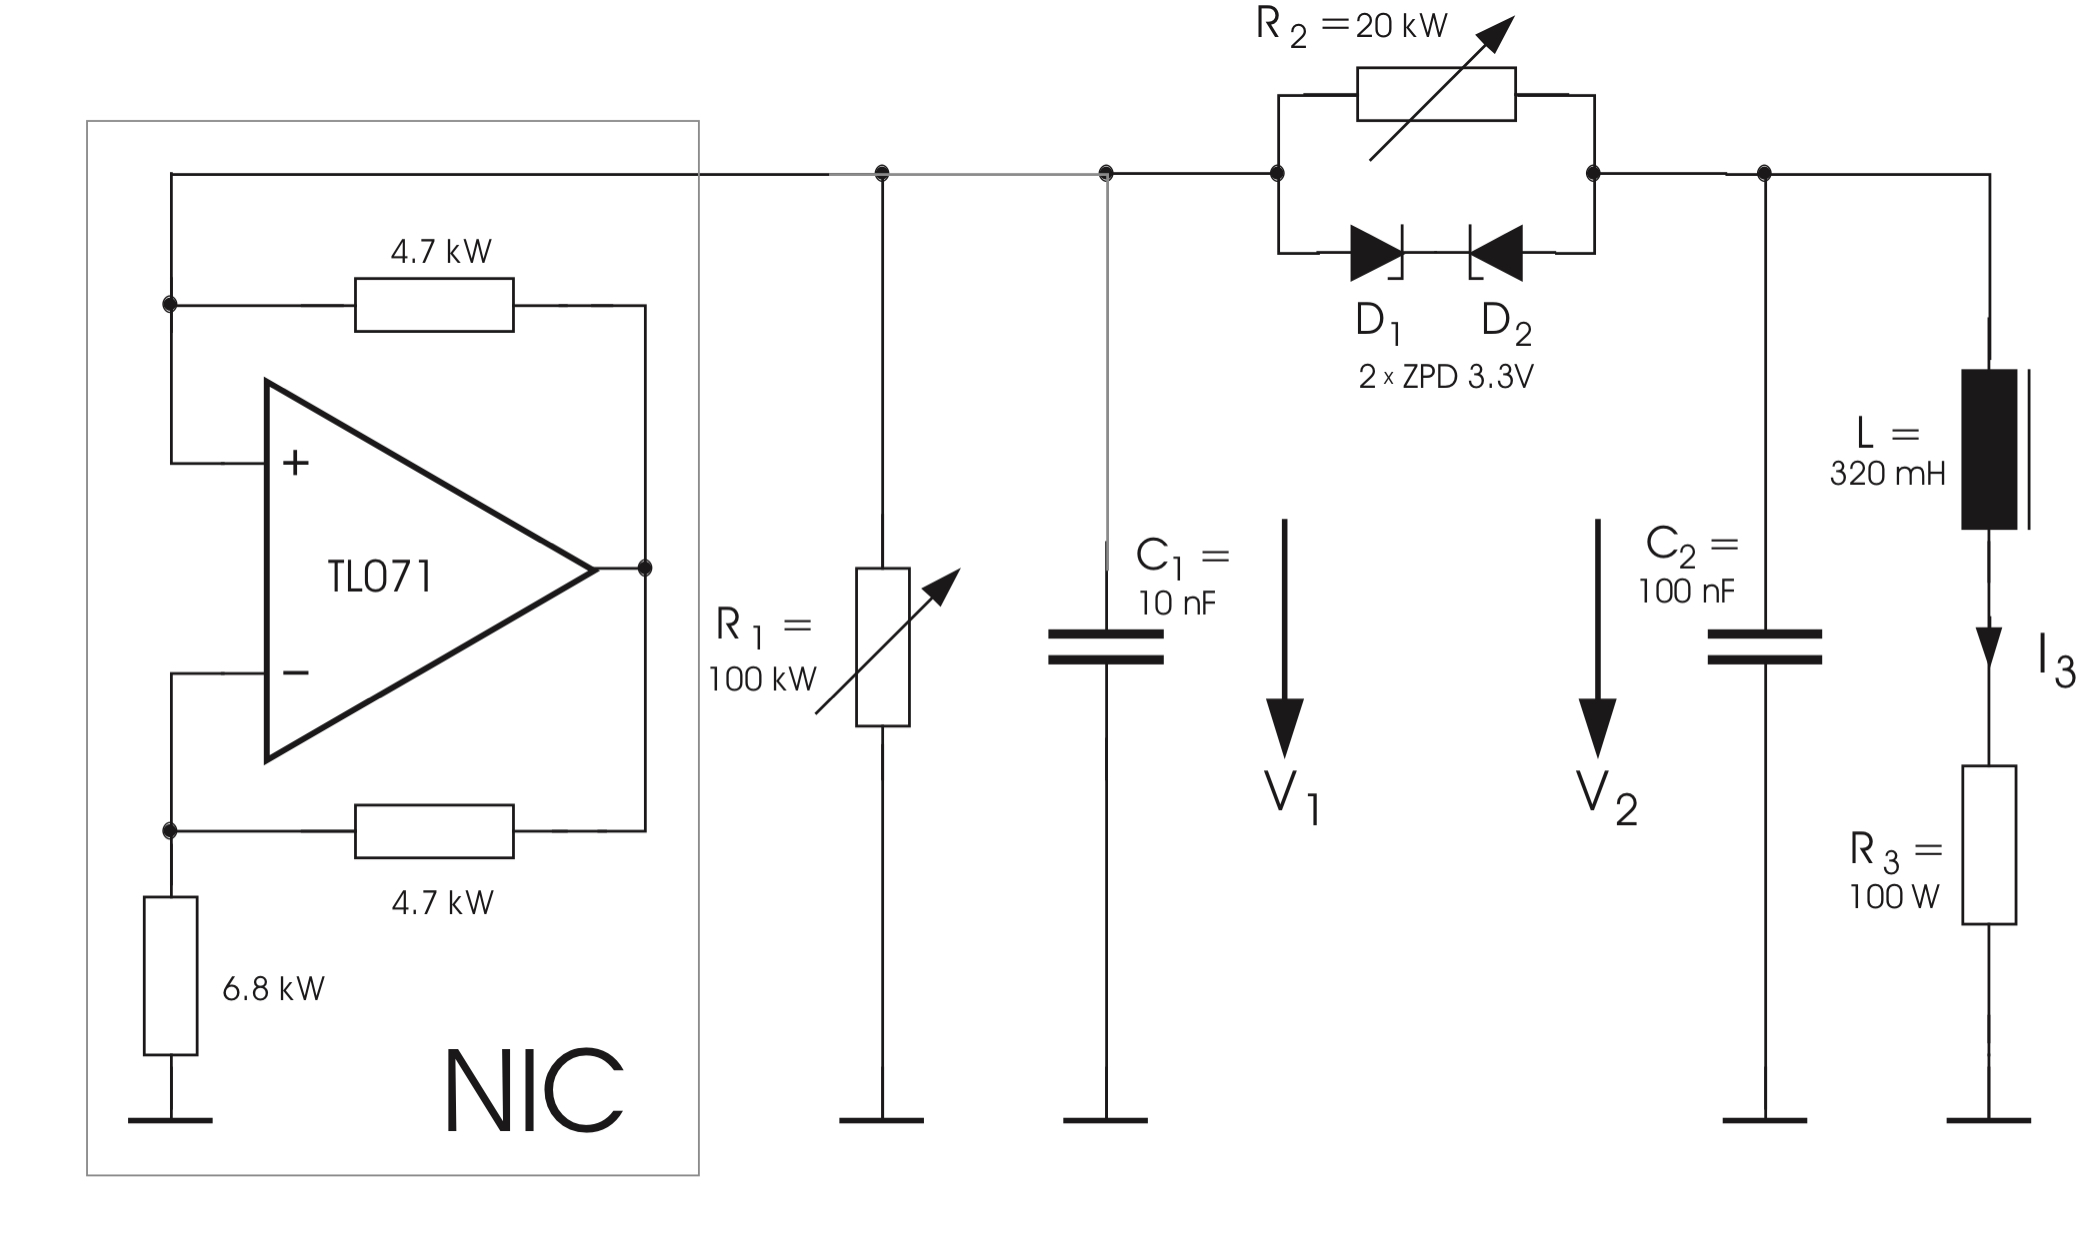
\includegraphics[scale=0.15]{ShinrOsziSp.jpeg}
    \label{fig:shinrikiSp}
    \caption{Schaltplan des Shinriki-Oszilator}
\end{figure}
% TODO: #25 Aufbau Shinriki @PaulSchwanitz

\subsection{Aufgabe: Shinrike}
\textbf{a) Phasendiagramm}\\
Wir stellen einzelne Paramterwerte für $R_2$ und $R_1$ ein und varieren je nach eingestellten Parameter mit $R_2$ oder $R_1$ bis das Phasendiagramm vollständig abgefahren ist ab. Widerstände schwer ablesbar, weswegen Angaben fehlerhaft sein können, $R_1$ konnte hierbei genauer bestimmt werden. Alle Werte werden in $\text{k}\Omega$ angeben.\\
\begin{tabular}{c  r| c  r  r  r  r  r  r  r}
    Par &  & Var & Per1 & Per2 & Per4 & Chaos1 & Per3 & Chaos2 & Double\\
    \hline
    $R_2$ & 16,50 & $R_1$ & 13,40 & 20,10 & 21,10 & 21,46 & 22,20 & 22,30 & 24,62\\
    $R_2$ & 13,00 & $R_1$ & 16,16 & 23,68 & 25,19 & 25,86 & 26,72 & 26,82 & 28,98\\
    $R_1$ & 55,00 & $R_2$ & 7,88  & 8,52 & 8,72 & 8,76 & 8,92 & 8,96 & 9,16\\
\end{tabular}\\

\textbf{b) Schnitt im Phasendiagramm}\\
Wir schneiden bei fixierten $R_2=8,4~\text{k}\Omega$ durch das Phasendiagramm.
Daten werden elektronisch erstellt.

\textbf{c) Bifurkationsdiagramm}\\
Nutzen oben verwendeten Schnitt für diese Aufgabe zum Erstellen eines Bifurkationsdiagramms. Dies geschieht wieder elektronisch.

\textbf{d) Großmann-Feigenbaum-Konstante}\\
Wir vermessen nun gesondert die einzelnen Bifurkationen durch Variation von $R_1$ mit gleichen $R_2$ aus (b). Alle Werte werden $\text{k}\Omega$ angegeben. Hierbei steht der Index $i$ in $r_i$ für die einzeln Bifurkationen.\\
\begin{tabular}{c c c}
    $r_1$ & $r_2$ & $r_3$\\
    \hline
    59 & 65,6 & 67,6
\end{tabular}

\textbf{e) Einbettungstheorem}\\
Aufnahme des Originalattraktors bei $R_2$ wie in (b) und $R_1=51~\text{k}\Omega$ und $\delta t=60$ n (?); Rekonstruktion mithilfe des entsprechenden Programmteils mit qualitativen Übereinstimmung der Form des rekonstruierten Attraktors mit dem Originalattraktor.

\section{Versuchsdurchführung}
\label{sec:durchfuehrung}

% Einbindung des Protokolls als pdf (mit Seitenzahl etc.)
% Erste Seite mit Überschrift
%\includepdf[pages = 1, landscape = false, nup = 1x1, scale = \skalierung , pagecommand={\thispagestyle{empty}\chapter{Protokoll}}]
%            {03-Protokoll/Protokoll.pdf}
% Restliche Seiten richtig skaliert
%\includepdf[pages = -, landscape = false, nup = 1x1, scale = \skalierung , pagecommand={}]
%            {03-Protokoll/Protokoll.pdf}